\chapter{Designing a white box model for collaborative filtering}\label{chapter:whitebox}

In this chapter we will describe our approach to design a white box\index{white box} model for collaborative filtering\index{collaborative filtering}. In order to provide explanations about the recommendation process, we will base our design on the characteristics of collaborative filtering.

\section{The visualization}\label{chapter:whitebox:section:visualization}

The underlying structure of collaborative filtering, the utility matrix, can be interpreted as a \emph{dual graph}\index{dual graph}. This is a graph $G(V,E)$ for which $V = U \cup I$ such that $U \cap I = \emptyset \wedge E \subseteq U \times I$\cite{dekimpe:2007}. Each non-blank entry in the utility matrix will then correspond to an edge. Figure \ref{figure:dualgraph} shows how a matrix is transformed into a dual graph.

When applied to the context of collaborative filtering, the set of nodes $U$ corresponds to the set of users, and the other set of nodes $I$ is set of items. In conclusion this means that there only exist edges of that go from an item to a user or from a user to an item.

\begin{figure}%
	\begin{center}
		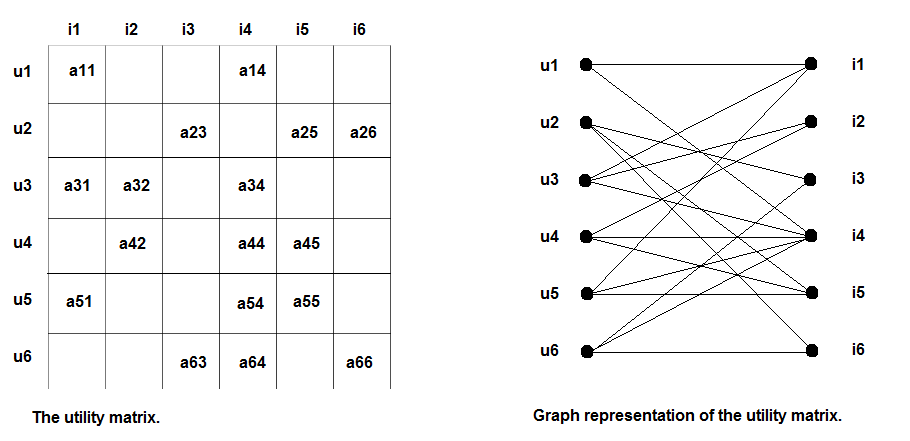
\includegraphics[width=300px]{img/dualgraph}
	\end{center}
	\caption{Transforming the utility matrix into a dual graph: two distinct sets of nodes, users and items, only share edges between nodes of different sets.}%
	\label{figure:dualgraph}%
\end{figure}

One of the challenges of this approach is overcoming the graph drawing problem, as defined earlier in section \ref{chapter:literature_study:section:interaction:subsection:graphs}. In an application where easily millions of items may be involved, scalability becomes a significant constraint on the visualization design\cite{herman:2000}.

Several strategies have been identified to reduce the number of items, reduce the number of dimensions and reduce visual clutter, as listed in section \ref{chapter:literature_study:section:interaction:subsection:techniques:subsubsection:reduction} and \ref{chapter:literature_study:section:interaction:subsection:graphs:subsubsection:reduction}.

Based on a visualization design by Valdis Krebs in \cite{steele:2010}, a dimensionality reduction\index{dimensionality reduction} can be performed on the dual graph, by keeping only one set of nodes and representing the other set of nodes as implicit information in the edges. Figure \ref{figure:rowreduction} shows an example of this idea of 'row reduction'\index{row reduction}. In Krebs' visualization the items, books purchased from the Amazon web store in this case, were retained. In the resulting graph, two items would share an edge if a user bought both these items. The thickness of the edges represented the number of users that where linked to these items\cite{krebs:2012:networkthinkers, steele:2010}.

\begin{figure}%
	\begin{center}
		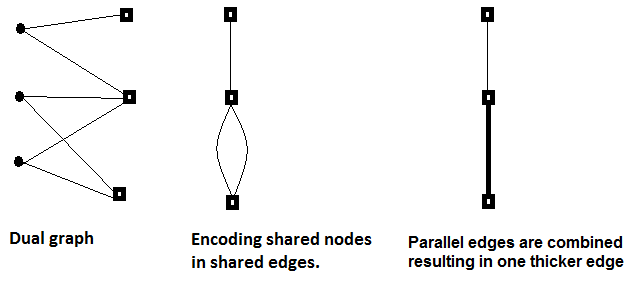
\includegraphics[width=250px]{img/row_reduction}%
	\end{center}
	\caption{A row reduction operation on each pair of edges in a dual graph will result in a dimensionality reduction where one set of nodes is removed from the graph.}%
	\label{figure:rowreduction}%
\end{figure}

For this white box model we will not apply the final step of Krebs' graph design. Instead we will keep parallel edges to keep a direct link between user and edge. In the resulting visualization of the CF-based recommender, a quantification of the similarity between users can then be established by counting parallel edges between items that occur in neighbouring profiles. Figure \ref{figure:rowreduction_dualgraph} shows how the dual graph from figure \ref{figure:dualgraph} is transformed into a circular graph layout with the remaining item nodes.

\begin{figure}%
	\begin{center}
		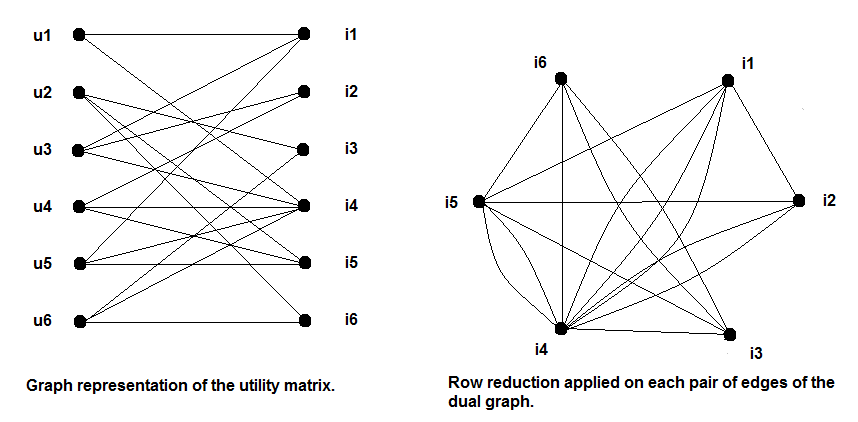
\includegraphics[width=250px]{img/dualgraph_rowreduction}%
	\end{center}
	\caption{Row reduction applied on the graph in figure \ref{figure:dualgraph}.}%
	\label{figure:rowreduction_dualgraph}%
\end{figure}

As it is unlikely that the whole user profile can be shown in the graph while avoiding visual clutter, the active user's favourite items are used to give a representation of the active user's profile. This way the user can still directly compare him/herself with neighbouring profiles. Due to the sparsity of the utility matrix, we might have to cluster multiple neighbouring profiles in a single node to ensure adequate connectivity within the graph.

Next we will apply edge-bundling on the graph to improve discernability and reduce visual clutter\cite{Holten:2006:HEB:1187627.1187772, holten:2009}. Figure \ref{figure:edgebundling_dualgraph} shows how this applied on the graph from figure \ref{figure:rowreduction_dualgraph}.

\begin{figure}%
	\begin{center}
		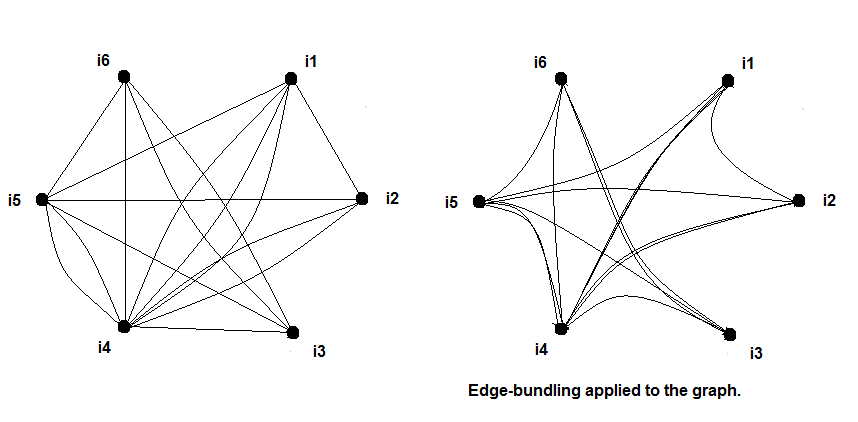
\includegraphics[width=250px]{img/dualgraph_edgebundling}%
	\end{center}
	\caption{Edge bundling applied on the graph in figure \ref{figure:rowreduction_dualgraph}.}%
	\label{figure:edgebundling_dualgraph}%
\end{figure}

From a graph drawing perspective we managed to reduce visual clutter by reducing the number of displayed items and applying edge-bundling\cite{herman:2000, Holten:2006:HEB:1187627.1187772}.  Of course cognitive aspects come into play as the visualization encodes now more implicit information that needs to be interpreted by the end user\cite{herman:2000, ware:2004}.

In order gain insight into the recommendation process, it is important that certain contextual information does not get lost through dimensionality and data reduction techniques. The contextual information we want to convey is two-fold:

\begin{enumerate}
	\item The strength of the links between a recommendation and the user's profile;
	\item The position of the user in his/her neighbourhood and the relation with those neighbours.
\end{enumerate}

% interaction techniques
To accomplish this, the active user's neighbours should be included in the visualization in one way or the other. One solution would be to label each of the edges with the corresponding neighbour's username. However, neighbour names may overlap each other, or occlude parts of the graph. Another idea would be similar to the PeerChooser application's layout. Re-introducing neighbours into the graph

Instead the user's top neighbours are listed next to the graph. By hovering or clicking one of the listed neighbours, the relevant parts of the graph, i.e., items owned by the neighbour and the edges between them, are highlighted.

% other design similar to PeerChooser: active user in the graph, his/her items directly around him. Neighbours are added or removed to the graph as desired.



\section{The visual thinking algorithm}\label{chapter:whitebox:section:algorithm}

We will try to approximate a visual thinking algorithm\index{visual thinking algorithm} applied by users when exploring the graph presented in section \ref{chapter:whitebox:section:visualization}. The algorithm in table \ref{table:visual_thinking_algorithm} is the degree-of-relevance highlighting algorithm derived by Ware and Mitchell \cite{ware:2004}.

\begin{table}
	\textit{Display environment: A display containing many symbols representing entities linked by a complex set of relationships.}

	\begin{enumerate}
		\item \textit{Construct a visual query to find a symbol that may lead to useful information (infromation scent).}
		\item \textit{Execute an epistemic action by selecting a symbol.} A symbol corresponds to either a user from the user list, or node on the graph.
		\item \textit{Computer highlights all symbols with a high degree of relevance to the selected symbol.} These are relevant parts of the graph, i.e., items owned by the neighbour and the edges between them, are highlighted.
		\item \textit{Execute a visual pattern query among the highlighted symbols for additional information scent.}
		\item \textit{If a very high relevance symbol is found, execute an epistemic action to drill down for additional information. Usually this will be presented in a different display window.} In this window artist and user metadata are shown, for example artist playcount, shared top artists et cetera.
		\item \textit{Repeat from step 1 as needed, cognitively marking visited symbols.}
	\end{enumerate}
\caption{Degree-of-relevance highlighting visual thinking algorithm by Ware and Mitchell \cite{ware:2004}.}
\label{table:visual_thinking_algorithm}
\end{table}





